\documentclass{deliverablereport}

\usepackage[style=alphabetic,backend=bibtex]{biblatex}
\addbibresource{../../lib/kbibs/kwarc.bib}
\addbibresource{../../lib/deliverables.bib}
\addbibresource{rest.bib}
% temporary fix due to http://tex.stackexchange.com/questions/311426/bibliography-error-use-of-blxbblverbaddi-doesnt-match-its-definition-ve
\makeatletter\def\blx@maxline{77}\makeatother

\usepackage{tikz}
\usepackage{standalone}
\usepackage[show]{ed}
\usepackage{listings}
\lstset{columns=fullflexible,basicstyle=\sf}
% Variant: we could just provide the deliverable label as in the
% proposal, and fetch all the information from final.pdata

\usepackage{listings}
\usepackage{graphicx}
\usepackage{float}

\usepackage{color}
\definecolor{gray}{rgb}{0.4,0.4,0.4}
\definecolor{darkblue}{rgb}{0.0,0.0,0.6}
\definecolor{cyan}{rgb}{0.0,0.6,0.6}

\lstset{
  basicstyle=\ttfamily,
  columns=fullflexible,
  showstringspaces=false,
  commentstyle=\color{gray}\upshape
}

\lstdefinelanguage{XML}
{
  morestring=[b]",
  morestring=[s]{>}{<},
  morecomment=[s]{<?}{?>},
  stringstyle=\color{black},
  identifierstyle=\color{darkblue},
  keywordstyle=\color{cyan},
  morekeywords={xmlns,version}
}

\deliverable{dksbases}{mws}
\issue{133}
\deliverydate{14/06/2016}
\duedate{1/07/2016 (M1)}
\def\pn{OpenDreamKit\xspace}

\def\MWS{\textsf{MathWebSearch}\xspace}

\author{Michael Kohlhase \& Alexandru Glontaru}

\usepackage[parfill]{parskip}
\begin{document}
\maketitle\vfill
\begin{abstract}
  A virtual research environment (VRE) contains extensive data (D), representations of
  knowledge (K), and software (S). This only becomes accessible to users, if the VRE
  provides a unified search facility for D/K/S structures. In the mathematical VRE under
  development in the \pn project, we have mathematical D/K/S, so that conventional search
  engines only partially apply. 

  In this report, we present the \MWS engine, an open-source, open-format,
  content-oriented full-text search engine for mathematical formulae encoded in Content
  MathML. We eventually want to use it for searching notebooks, active documents and the
  Math-in-the-Middle Ontology in the \pn VRE. This report only presents the current system
  that can search mathematical documents written in {\LaTeX} or HTML5. 

%   \MWS is a complete system capable of crawling, indexing, and querying
%   expressions based on their functional structure (operator tree) rather than their
%   presentation. It combines a powerful exact formula unification/matching with the
%   fulltext search capabilities of ElasticSearch to achieve simultaneous full-text search
%   for mathematical/technical documents. 

%   \MWS focuses on scalability (memory footprint, index persistence), integration of
%   keyword- and formula search, and hit presentation issues. It forms a stable basis for
%   future research into extended query languages and user-interaction issues. The system
%   has been integrated into high-profile information systems like Zentralblatt Math.
 
% The software is licensed under the GNU General Public License version 3. 
 \end{abstract}
\vfill
\newpage\tableofcontents\newpage

\section{Introduction: Search in \pn}

A virtual research environment (VRE) contains extensive data (D), representations of
knowledge (K), and software (S). This only becomes accessible to users, if the VRE
provides a unified search facility for D/K/S structures. In the mathematical VRE under
development in the \pn project, we have mathematical D/K/S, so that conventional search
engines only partially apply. 

In this report, we present the \MWS engine, an open-source, open-format,
content-oriented full-text search engine for mathematical formulae encoded in Content
MathML. We eventually want to use it for searching notebooks, active documents and the
Math-in-the-Middle Ontology in the \pn VRE. This report only presents the current system
that can search mathematical documents written in {\LaTeX} or HTML5. For applications to
other D/K/S structures, see Section~\ref{sec:concl}.
 
The report is organized as follows: in Section~\ref{sec:mws} we give a general overview
over the \MWS system as a base for a discussion of the system's components in the
ensuing sections: Sections~\ref{sec:harvests} and \ref{sec:ml} discuss the input format
(MWS harvests) and how to convert {\TeX/\LaTeX} documents so that they can be
harvested. Sections~\ref{sec:mathindex} to \ref{distribution} give an overview over
internals of the \MWS backend: indexing of formulae and full text, and
distributed querying. Section~\ref{frontend} presents a web front-end for \MWS
and Section~\ref{sec:arxiv} discusses the larger corpora the system is used for.
Section~\ref{sec:concl} concludes the report and details future work.

\section{\MWS Overview}\label{sec:mws}

Mathematics-aware information retrieval (MIR) has often been touted as one of the “killer
applications” of computer support in STEM (Science, Technology, Engineering, and
Mathematics). Indeed, the yearly production of published research in mathematics exceeds
120 thousand journal articles a year alone~\cite{KohProHam:ntcir11}; the amount of
internal technical documents in company archives certainly exceeds this quantity by far;
being able to access the knowledge locked up in them will become a determining factor for
commercial success.

MWS is a web application that provides low-latency answers to full-text queries which
consist of keywords and formulae. \MWS front-ends convert formula schemata (with query
variables) into content MathML expressions, which the \MWS formula indexer answers by
unification and combines the results with keyword results from a text search engine. The
modular architecture and standardized formats makes \MWS applicable to a wide range of
querying tasks – web-based formula search engines or editing support services. Unification
queries over content MathML expressions form the basis of an expressive query language
with well-defined semantics. As substitution instances of the original query, \MWS results
are highly significant, if the encoding of data set and search query are adequate –
i.e. do not drop or spuriously introduce salient semantic
features~\cite{KohProHam:ntcir11}.

At its core, the \MWS system is a content-based search engine for mathematical
formulae. It indexes MathML formulae, using a technique derived from automated theorem
proving: Substitution Tree Indexing. Recently, it was augmented with full-text search
capabilities, combining keyword queries with unification-based formula search. The engine
serving text queries is Elasticsearch 2.3. From now on, in order to avoid confusion, we
will refer to the core system (providing just formula query capability) as \MWS and to the
complete service (MWS + Elasticsearch) as TeMaSearch (Text + Math Search).

The overall workflow of TeMaSearch is the following~\cite{Ham:bcs15}: 

\begin{enumerate}
\item HTML5 documents representing mathematical articles are crawled to generate \MWS
  harvests. The harvest format is an extension of MathML which \MWS can index. Its role is
  to separate the math from the text in a given document.
\item \MWS indexes the harvests.
\item a second pass is made over the harvests to generate annotated documents.
\item Elasticsearch indexes the annotated documents.
\item Everything is now ready for answering queries. When a query is issued, \MWS will
  answer the mathematical part and Elasticsearch will answer the text part. The results
  are combined through a NodeJS proxy to send a final result set.
\end{enumerate}

Each mathematical expression is encoded as a set of substitutions based on a depth-first
traversal of its Content MathML tree. Furthermore, each tag from the Content MathML tree
is encoded as a TokenID, to lower the size of the resulting index. The (bijective) mapping
is also stored together with the index and is needed to reconstruct the original
formula. The index itself is an in-memory trie of substitution paths.

To facilitate fast retrieval, \MWS stores FormulaIDs in the leaves of the substitution
tree. These are integers uniquely associated with formulae, and they are used to store the
context in which the respective expressions occurred. These identifiers are stored in a
separate LevelDB database.

\section{MwsHarvests}\label{sec:harvests}

MwsHarvests is the format that the \MWS accepts as crawled data. It is an
extension of MathML which introduces a few tags and attributes to specify meta-information
about the crawled Content MathML data~\cite{MWSH}.

The introduced tags are \textbf{\texttt{harvest}}, \textbf{\texttt{expr}} and
\textbf{\texttt{data}}, all defined in the mws namespace. The root element of a MwsHarvest
is a \textbf{\texttt{mws:harvest}}. Its children are \textbf{\texttt{mws:expr}} and
\textbf{\texttt{mws:data}} nodes. \textbf{\texttt{mws:expr}} nodes contain the actual
ContentMathML and have the following attributes:

\begin{itemize}
\item \textbf{\texttt{url}} specifies the URL+UUID of the \textbf{\texttt{m:math}} from
  which the content was extracted,
\item \textbf{\texttt{data\_id}} specifies the \textbf{\texttt{id}} of a
  \textbf{\texttt{mws:data}} node previously defined in this document. The respective data
  will be associated with this expression.
\end{itemize}

\textbf{\texttt{mws:data}} nodes contain arbitrary XML data and have the following
attributes:
\begin{itemize}
\item \textbf{\texttt{data\_id}} specifies an unique identifier within this XML document.
\end{itemize}

Note that \textbf{\texttt{mws:data}} has been introduced in version 2 of the
\textbf{\texttt{mws:harvest}}, but it is backward compatible.

An example harvest document is provided here:

\lstset{language=XML,basicstyle=\footnotesize\sf}
\begin{lstlisting}
<?xml version="1.0"?>
<mws:harvest xmlns:mws="http://search.mathweb.org/ns" 
			xmlns:m="http://www.w3.org/1998/Math/MathML">
    <mws:data mws:data_id="foo">
       <!-- arbitrary XML data -->
    </mws:data>
    <mws:expr url="http://math.example.org/article123456#e123456"
    			mws:data_id="foo">
        <m:apply>
            <m:eq/>
            <m:apply>
                <m:apply>
                    <m:csymbol cd="ambiguous">subscript</m:csymbol>
                    <m:limit/>
                    <m:apply>
                        <m:ci>&#x2192;</m:ci>
                        <m:ci>x</m:ci>
                        <m:cn>0</m:cn>
                    </m:apply>
                </m:apply>
                <m:apply>
                    <m:divide/>
                    <m:cn>1</m:cn>
                    <m:apply>
                        <m:csymbol cd="ambiguous">superscript</m:csymbol>
                        <m:ci>x</m:ci>
                        <m:cn>2</m:cn>
                    </m:apply>
                </m:apply>
            </m:apply>
            <m:infinity/>
        </m:apply>
    </mws:expr>
    <!--
        More mws:data and mws:expr nodes
    -->
</mws:harvest>
\end{lstlisting}

This specifies that the data contained in the \textbf{\texttt{mws:expr}} was extracted from an \textbf{\texttt{m:math}} node found in the document \url{http://math.example.org/article123456} with id e123456.

\section{LATEXML}\label{sec:ml}
An overwhelming majority of the digital scientific content is written using LATEX or TEX,
due to its usability and popularity among STEM researchers. However, formulae in these
formats are not good candidates for searching because they do not display the mathematical
structure of the underlying idea. For this purpose, conversion engines have been developed
to convert LATEX expressions to more organized formats such as MathML~\cite{Ham:bcs15}.

An open source example of such a conversion engine is LATEXML. The \MWS project
relies heavily on it, to convert arXiv documents from LATEX to XHTML which is later
indexed by \MWS. It exposes a powerful API, accepting custom definition files which relate
TEX elements to corresponding XML fragments that should be generated. For the scope of
this project, we are more interested in another feature of LATEXML: cross-referencing
between Presentation MathML and Content MathML. While converting TEX entities to
Presentation MathML trees, LATEXML assigns each PMML element a unique identifier which is
later referenced from the corresponding Con-tent MathML element. In this manner, we can
modify the Content MathML tree and reflect the changes in the Presentation MathML tree
which can be displayed to the user.
 

\begin{figure}[h]
\centering
 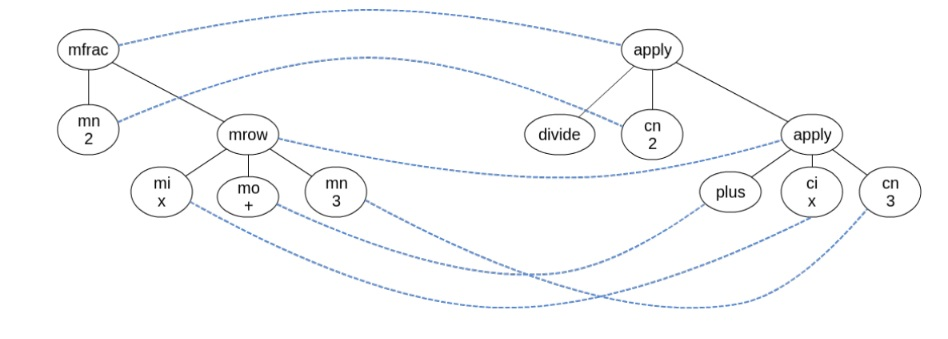
\includegraphics[scale=0.6]{figure2.jpg}
 \caption{The CMML/PMML Parallel Markup}
 \label{fig:markup}
\end{figure}

Figure~\ref{fig:markup} illustrates the parallel markup for 2 Presentation MathML and on the right side,
Content MathML. As we can see, every Content element has a Presentation correspondent,
except the divide operator, whose meaning is reflected in the structure of the displayed
formula. On the left side we have Presentation MathML and on the right side, Content
MathML. As we can see, every Content element has a Presentation correspondent, except the
divide operator, whose meaning is reflected in the structure of the displayed formula.



\section{Indexing Mathematical Formulae}\label{sec:mathindex}

For indexing mathematical formulae on the web, we will interpret them as first-order
terms. This allows us to use a technique from automated reasoning called term
indexing. This is the process by which a set of terms is stored in a special purpose data
structure (the index, normally stored in memory) where common parts of the terms are
potentially shared, so as to minimize access time and storage. The indexing technique we
work with is a form of tree-based indexing called substitution-tree indexing~\cite{KohSuc:asemf06}. A
substitution tree, as the name suggests, is simply a tree where substitutions are the
nodes. A term is constructed by successively applying substitutions along a path in the
tree, the leaves represent the terms stored in the index. Internal nodes of the tree are
generic terms and represent similarities between terms.

\begin{figure}[h]
\centering
 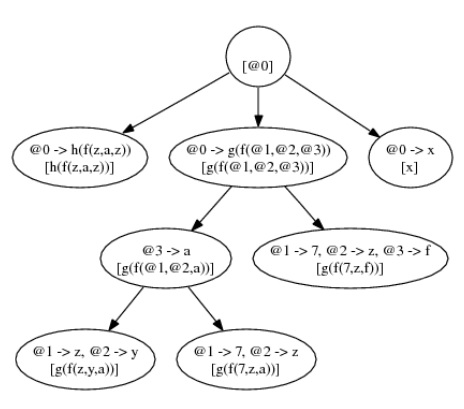
\includegraphics[scale=0.9]{figure1.jpg}
 \caption{Division Tree Example}
 \label{fig:tree}
\end{figure}

The main advantage of substitution tree indexing is that we only store substitutions, not
the actual terms, and this leads to a small memory footprint. Figure~\ref{fig:tree} shows a typical
index for the terms $h(f(z, a, z))$, $x$, $g(f(z, y, a))$, $g(f(7, z, a))$, and
$g(f(7, z, f))$. For clarity we present not only the substitutions in the node, but the
term produced up to that node as well (between square brackets). The variables @integer
are used to denote placeholder variables for parts that differ between terms. All
placeholder variables are substituted before a leaf is reached.

Adding data to an existing index is simple and fast, querying the data structure is
reduced to performing a walk down the tree. In contrast to automated reasoning our
application does not need tree merging. Therefore we use substitutions only when building
the index. Index building is done based on Algorithm 1. Once the index is built, we keep
the actual term instead of the substitution at each node, so we do not have to recompute
it with every search. Structure sharing methods conserve memory and make this
tractable. To each of the indexed terms, some data is attached — an identifier that
relates the term to its exact location. The identifier, location and other relevant data
are stored in a database external to the search engine. We use XPointer references to
specify term locations.

Unfortunately, substitution tree indexing does not support subterm search in an elegant
fashion, so when adding a term to the index, we add all its subterms as well. This simple
trick works well: the increase in index size remains manageable and it greatly simplifies
the implementation. The rather small increase is caused by the fact that many of the
subterms are shared among larger terms and they are only added once.

\section{Elastic Search}\label{sec:elastic}
Elasticsearch is a powerful and efficient full text search and analytics engine, built on
top of Lucene~\cite{Elastic}. It can scale massively, because it partitions data in shards and is also
fault tolerant, because it replicates data. It indexes schema-free JSON documents and the
search engine exposes a REST-ful web interface. The query is also structured as JSON and
supports a multitude of features via its domain specific language: nested queries,
filters, ranking, scoring, searching using wildcards/ranges and faceted search.

The faceted search feature \footnote{Faceted search as such is now deprecated in ES and
  was replaced by the more powerful “aggregations” feature, which also allows facets of
  facets, i.e. nested facets.} this feature is the terms aggregation: a multi-bucket
aggregation, with dynamically built buckets. We can specify an array field from a document
and ask ES to count how many unique items from the array are there in the whole
index. This list can also be sorted, e.g. most frequently occurring items
first. Additionally, we can also impose a limit on the number of the buckets (items) for
which we want to receive the count. is of particular interest to us. One way to use this
feature is the terms aggregation: a multi-bucket aggregation, with dynamically built
buckets. We can specify an array field from a document and ask ES to count how many unique
items from the array are there in the whole index. This list can also be sorted, e.g. most
frequently occurring items first. Additionally, we can also impose a limit on the number
of the buckets (items) for which we want to receive the count.

\begin{lstlisting}[caption={Elastic Search Term Aggregation Query}\label{listone}]
{
	"query" : {
		"match" : {
			"body" : {
				"query" : "Pierre Fermat",
				"operator" : "and"
			}
		}
	},

	"aggs" : {
		"formulae" : {
			"terms" : { "field" : "ids" }
		}
	}
}

\end{lstlisting}

An ES query which would return the most frequently used formulae (and subformulae) for
“Pierre Fermat”, is presented in Listing~\ref{listone}. The key part is the aggs fields. We are
specifying that we want an aggregation called Formulae on “terms” (i.e. we want bucket
counting) and the target of the aggregation is the fields ids. 

A possible response to the above query can be found in Listing~\ref{listtwo}. In the response we can
see the returned aggregations. In our example there is only one and it is called
formulae. We can find the actual result in the buckets field. The key field in the bucket
corresponds to a FormulaID. Here, the most frequent formulae were the one with ID 230 and
the one with ID 93. The former appeared in 10 documents and the latter appeared in 9
documents.

\begin{lstlisting}[caption={Elastic Search Term Aggregation Response}\label{listtwo}]
{
	...
	"aggregations" : {
		"formulae" : {
			"buckets" : [
			{
				"key" : "230",
				"doc_count" : 10
			},
			{
				"key" : "93",
				"doc_count" : 9
			},
			...
			]
		}
	}
}
\end{lstlisting}

\section{Integration via the Query Proxy}\label{sec:proxy}

The query proxy is a HTTP RESTful interface which provides text and formula search. It is the operational heart of the full-text search functionality that is new for the NTCIR-11 version of \MWS. As we show in figure~\ref{fig:markup2}, its backend is a \MWS formula indexer serving the formula index and an ElasticSearch daemon serving the annotated documents. 

Upon receiving a query, it sends the formula to the formula indexer service and receives the matching formula identifiers. Using these, along with the text query, it queries ElasticSearch for documents which contain the respective text and the formula identifiers. As these documents may be large, only their unique identifiers are retrieved and a secondary query is used to provide snippets with the relevant data. 

\begin{figure}[h]
\centering
 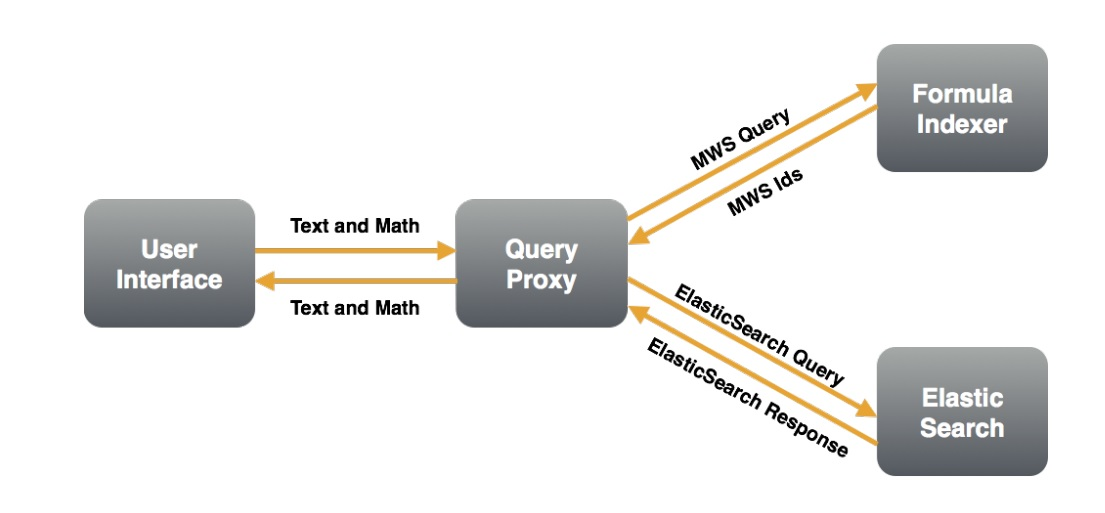
\includegraphics[scale=0.7]{figure3.jpg}
 \caption{The CMML/PMML Parallel Markup}
 \label{fig:markup2}
\end{figure}

Internally, we can configure what is considered a hit by manipulating the query we present to ElasticSearch. It understands an expressive language, allowing us to define a match as any document containing the formula, and (or) at least n or a percentage of words. In the current configuration, a document is considered a hit if it contains a formula matching the formula query and at least one of the words in the text query. 

\section{Distribution of Indexing and Querying}\label{distribution}
As presented above, the main indexing data structure is a DFS substitution tree. To represent the tree in a manner which supports cross-machine links, we use three types of index nodes:~\cite{ProKoh:mwsofse11}
 
\begin{enumerate}
\item \textbf{Internal Index Nodes} They are used to navigate through most parts of the tree. Their data stores mappings from token ID to the corresponding index node.
\item \textbf{Leaf Index Nodes} They represent the end of a particular formula and its corresponding ID in the URL+URI database.
\item \textbf{Remote Index Nodes} They represent cross-sector links. Their data consists of a pair of memory sector ID and node ID, which uniquely determine the corresponding index node.
\end{enumerate}
 
As harvests are fed into the system, the index is built. Notice that, instead of building it on the heap (with no control over individual node’s memory locations), the system places it inside specific memory sectors. 

Memory sectors are continuous areas of memory of fixed sizes, usually represented as memory mapped files. They are the smallest units of replication, migration, and load balancing. When the system starts, an initial memory sector is created and the tree is built in this area. As terms get inserted, the sector fills. When it reaches a given threshold, a new sector is created and the contents of the original sector get split between the two. 

In Figure~\ref{fig:memory_sectors}, we present an example of term insertion which causes a tree split. Consider the initial tree containing the expressions f(a) and b and Memory Sectors of size 12 units, as depicted in Figure~\ref{fig:memory_sectors}(a). We consider a memory model where each link and each node costs 1 unit. Let’s insert g(f(x)). As the resulting tree would overflow the current memory sector, a new one is created and parts of the tree are migrated to the new memory sector (See Figure~\ref{fig:memory_sectors}(b)). To split the tree, the system performs a DFS traversal, as long as the size needed to store the explored and queued nodes does not exceed a given threshold (in our case, 10). Once a node expansion would go over it, all the internal nodes in the queue are transformed into remote nodes and the rest is moved to the other memory sector. 

\begin{figure}[h]
\centering
 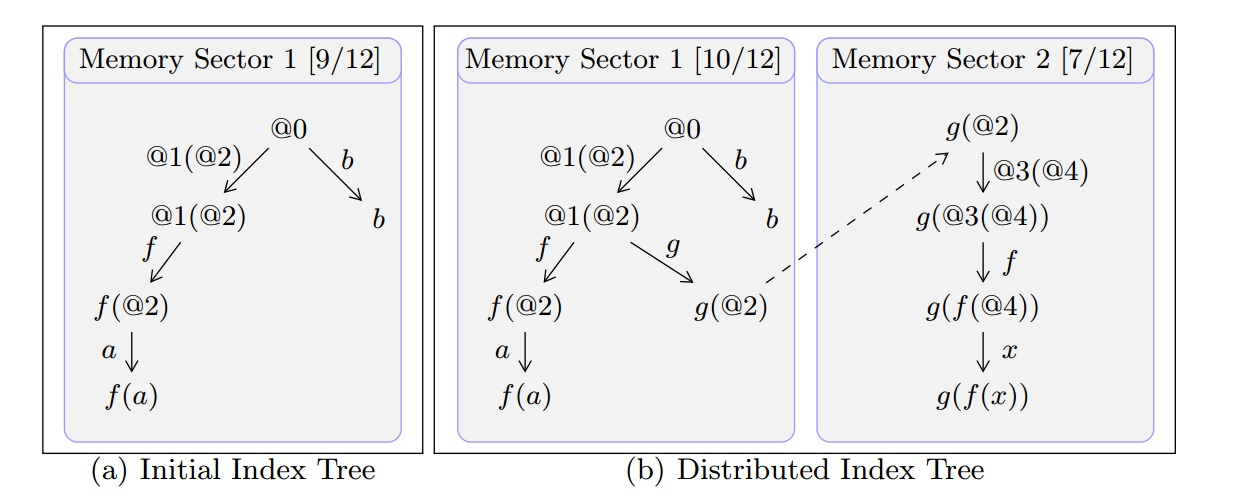
\includegraphics[scale=0.6]{figure4.jpg}
 \caption{Tree Distribution across Memory Sectors}
 \label{fig:memory_sectors}
\end{figure}

The advantage of the new data structures is that indexes can be distributed over multiple
computers: when the memory usage on one machine goes above a specific threshold, a
percentage of the memory sectors are migrated to other
machines~\cite{ProKoh:mwsofse11}. As the tree uses only relative pointers and the sectors
are represented as memory mapped files, it is enough to flush the memory sector to the
file, send it across the network, and re-map it into the new system’s memory (of course,
we assume endian-compatible machines). All operations on memory sectors (splits,
migrations) are coordinated by a master node, which keeps track of their locations, as
well as cross-sector links.

For a distributed instance of \MWS we have the following setup: All nodes in the network
of \MWS machines run \texttt{mwsd} (the \MWS daemon with the index and the URI
database). \MWS has only one \texttt{restd} daemon, which resides on the master node. Upon
receiving Q \texttt{restd} passes it to \texttt{mwsd} on the master node, which start DFS
search on its substitution tree index fragment. Whenever \texttt{mwsd} hits a remote index
node whose target sector is on a different machine, it forwards the respective subquery Q0
to the \texttt{mwsd} on the remote machine, while continuing processing on the current
machine.

In result-unlimited queries, the master \texttt{mwsd} will just wait for the slave
\texttt{mwsd} to return the results and aggregate that with its own result set. In
result-limited cases, some of the slave’s results may be irrelevant, since the result
limit has already been reached. The tradeoffs and efficiency issues involved in such
effects will still need to be investigated. Similarly, the top of the index tree (which
resides on the master node) will receive much higher processing loads, possibly becoming a
bottleneck to the overall system.


\section{Frontend}\label{frontend}
For exampling the functionality of \MWS we will continue by presenting two frontends based
on its mechanism. The first one is a text-only search engine which returns the math from
the matching documents, after running it through the schematizer (the core part of
MWS). This is the demo for showcasing the schematization process. The second one is a
direct application of the Schematizer into a Math Search Engine which is capable of
mathematical faceted search.~\cite{HamKoh:fsfm15}

\subsection{SchemaSearch}\label{shcemasearch}
The SchemaSearch front-end provides just a textual search input field. It is intended for
users who want an overview of the formulae contained in a corpus. As shown in figure
~\ref{fig:schema_search}, the user can enter a set of keywords for the query, as well as a
schema depth, which defaults to 3. The maximum result size is not accessible to the user,
to prevent abuses and reduce server load. There is also an “R” checkbox which specifies if
the cutoff depth should be absolute or relative. If relative, the depth should be given in
percentages~\cite{Ham:bcs15}.

\begin{figure}[h]
\centering
 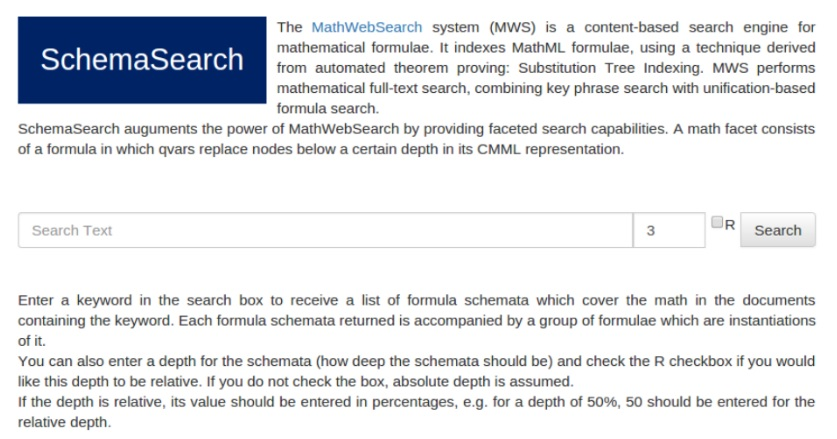
\includegraphics[scale=0.9]{figure5.jpg}
 \caption{SchemaSearch frontend}
 \label{fig:schema_search}
\end{figure}



\subsection{TemaV2 frontend}\label{v2}

The TemaV2 front-end extends TeMaSearch to be able to perform mathematical faceted
search. It is intended for users who want to filter query results based on a given facet
(formula schema in this case). The look and feel is similar to the previous version of
TeMaSearch, as shown in Figure~\ref{fig:temav2}, where the first input field is used to
specify keywords and the second one is used to specify LATEX-style formulae for the
query. When returning results, a “Math Facets” menu will be presented to the
user~\cite{Ham:bcs15}.

\begin{figure}[H]
\centering
 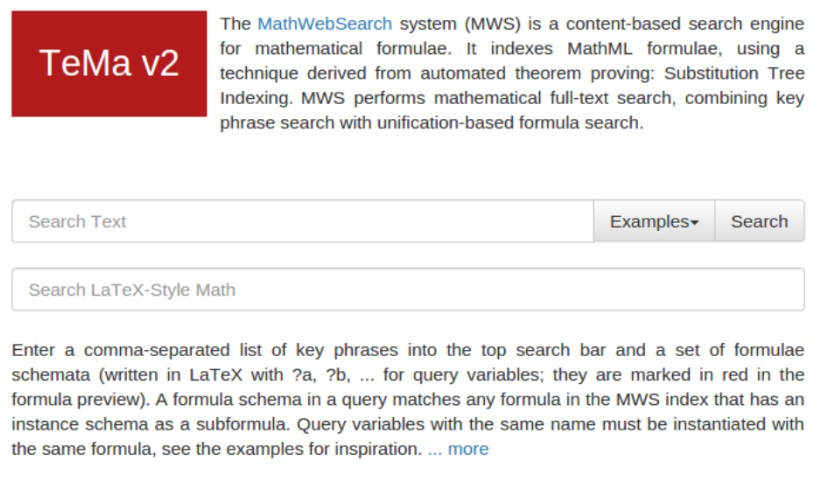
\includegraphics[scale=0.8]{figure6.jpg}
 \caption{TemaV2 frontend}
 \label{fig:temav2}
\end{figure}

Figure~\ref{fig:temav2query} shows the results of a query for “Fermat” and $?a^{?n}+?b^{?n}=?c^{?n}$.

\begin{figure}[H]
\centering
 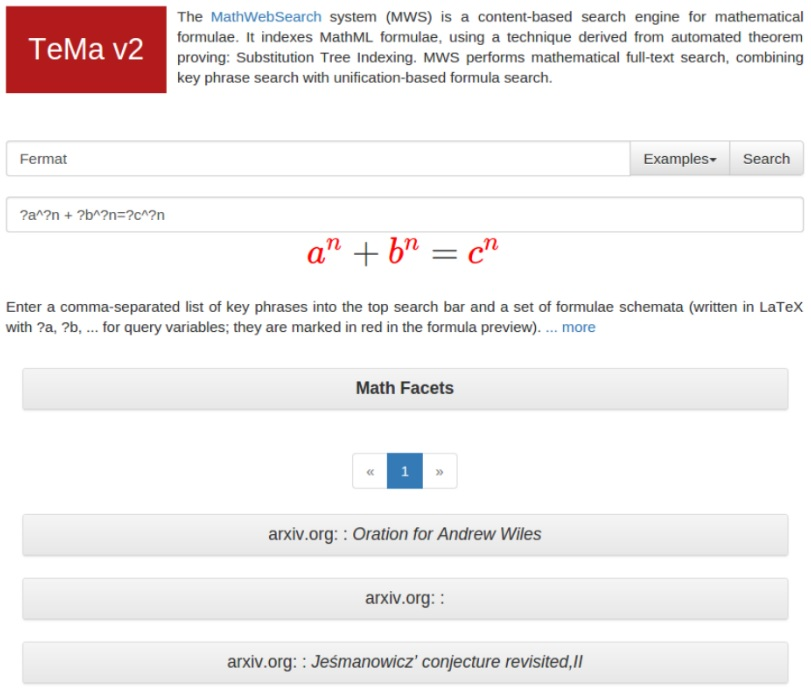
\includegraphics[scale=0.6]{figure7.jpg}
 \caption{TeMa v2 Query Results}
 \label{fig:temav2query}
\end{figure}


\section{\MWS Instances and Corpora: arXiv, ZBMath, Mizar}\label{arxiv}

The \MWS system has been used to supply search instances on various corpora of
mathematical documents, we describe three here, others can be seen on
\url{http://search.mathweb.org}. 

\subsection{arXiv search}

Begun on August 14, 1991, created by Paul Ginsparg, the ``Cornell e-Print arXiv''
(\url{http://arXiv.org}) is a repository of scientific papers and electronic preprints in
fields of mathematics, computer science, physics, astronomy, biology and statistics or
finance written in {\TeX/\LaTeX} for an optimized transfer over the internet and an easily
rendered client-side. In present the project is hosted by Cornell University and includes
over a million articles and increases with around 8000 per month.

The KWARC group have converted by arXiv corpus into HTML5~\cite{StaKoh:tlcspx10} and
harvested it for \MWS. The instance at \url{http://arxivsearch.mathweb.org}
indexes over 105\,000 math-heavy papers. This sub-corpus has also been used for the NTCIR
Math Information Retrieval
Challenges~\cite{AizKohOun:nmpto13,AizKohOunSch:nmto14,AizKohOunSch:nmto16}.

\subsection{zbMATH search}

Zentralblatt Math (zbMath) is a mathematical information service that curates a database
of reviews and classifications (MSC, see~\cite{MSC2010}) for all articles in mathematics
since the middle of the 19th century. The database currently contains 3.8 million reviews
and grows at a rate of ca 120\,000 reviews per year. The zbMATH portal at
\url{https://zbmath.org/} offers a faceted search engine for reviews based on
bibliographic metadata, MSC classification, and \emph{formulae}. The latter is driven by
\MWS.

\subsection{Search on a Formal Library of Mathematical Knowledge}

We have converted the Mizar Mathematical Library~\cite{MizarKB:on} to the OMDoc/MMT format
and indexed the results in \MWS~\cite{IanKohRabUrb:tmmliotaa13}, enabling
formula-based search on a formal knowledge of contains over 1000 articles with over 50000
theorems and over 10000 definitions encoded in first-order logic based on
Tarski-Grothendiek set theory. As the data is fully formal, we can identify universal
variables in the corpus (explicitly marked up universal quantifications) and search for
applicable theorems, e.g. we can issue queries like formula query:
\def\var#1{\textcolor{red}{?#1}} $\int_a^b |V(t)I(t)| dt\leq\var{R}$, and the \pn system
will return H\"older's equation as one of the hits:
\begin{quote}
  \textbf{Theorem 17.} (H\"older's Inequality)\\\it
  If $f$ and $g$ are measurable real functions, $l,h\in\mathbb{R}$, and  $p,q\in
  [0,\infty)$, such that $1/p + 1/q = 1$, then 
  \begin{equation}\label{eq:hi}
  \int_l^h \left|f(x)g(x)\right| dx \leq\kern-.4em 
    \left(\int_l^h\left|f(x)\right|^p dx\right)^\frac{1}{p} 
    \kern-.5em
    \left(\int_l^h\left|g(x)\right|^q dx \right)^\frac{1}{q}
  \end{equation}
\end{quote}

\section{Conclusion}\label{sec:concl}
We have presented a search engine capable of dealing with pure mathematical queries but
also with text and math queries. The \MWS web service is open source software released
under the GNU public license. The code is available from the developer
portal~\cite{MWS-git:on}. Search front-ends for various corpora and applications are
referenced on the \MWS project page~\cite{MWSProj:on}. In contrast to other
approaches, \MWS uses the full content structure of formulae and is easily
extensible to other content-oriented formats. Our evaluations show that query times are
low and essentially constant in index/harvest size, so that a search engine can scale up
to web proportions. Contrary to our expectations, index size is linear in harvest size for
the arXiv corpus, which transcends the main memory limits of standard servers. Therefore,
implementing parallelization/distribution strategies is a priority.

\subsection*{Adaptation to \pn} For utilization in the \pn VRE we need to solve two
development problems: 
\begin{compactenum}[\bf ODK1]
\item for all types of data (D), representations of knowledge (K), and software (S) in \pn
  we need \MWS harvesters -- i.e. systems that transform the D/K/S strutures into \MWS
  harvests (see Section~\ref{sec:harvests}).
\item for all interfaces in the \pn VRE -- see e.g.~\cite{ODK-D4.2} -- we need to embed
  search front-ends that make use of the user context to allow precise and convenient
  entry of queries and selection/ranking of search results.
\end{compactenum}
Work on these has already begun. For instance we have parsed the formulae in the ``Open
Encyclopedia of Integer Sequences'' (OEIS, see~\cite{oeis} and Task \textbf{T6.6} in the
\pn proposal) and harvested them for \MWS (\textbf{ODK1}) and built an OEIS-specific
front-end (\textbf{ODK2}), see~\cite{LuzKoh:fsarfo16}. Further more we are currently
working on exporting the D/K/S structures in the LMFDB, GAP, and SageMath into
\MWS-harvestable OMDoc/MMT format (\textbf{ODK1}). 

\newpage\printbibliography
\end{document}

%%% Local Variables:
%%% mode: latex
%%% TeX-master: t
%%% End:

%  LocalWords:  maketitle vfill pn newpage tableofcontents newpage concl organized mws cn
%  LocalWords:  arxiv standardized Elasticsearch bcs15 textbf textbf texttt itemize xmlns
%  LocalWords:  lstset lstlisting csymbol centering includegraphics asemf06 XPointer mwsd
%  LocalWords:  subterms Lucene listone subformulae listtwo mwsofse11 restd schematizer
%  LocalWords:  schematization fsfm15 shcemasearch qvars temav2 temav2query Mizar StaKoh
%  LocalWords:  Ginsparg optimized tlcspx10 AizKohOun nmpto13 AizKohOunSch nmto14 nmto16
%  LocalWords:  AizKohOunSch zbMATH emph IanKohRabUrb tmmliotaa13 Tarski-Grothendiek leq
%  LocalWords:  mathbb infty MWSProj parallelization utilization compactenum oeis LuzKoh
%  LocalWords:  fsarfo16 printbibliography
